\documentclass[11pt, a4paper]{article}

\usepackage[english]{babel}
\usepackage{sleek}
\usepackage[nosolutions]{common}

\title{Introduction to Artificial Intelligence (INFO8006)}
\subtitle{Exercise session 4}

\begin{document}

\def\var{\text{$\sigma^2$}}

\maketitle

% \begin{thbox}{d-separation}
    
% \end{thbox}

\begin{thbox}{Maximum likelihood estimation}
    Given a set of i.i.d. observations $\mathcal{D} = \{x_1,...,x_N\}$, a set of unknown \thighlight{parameters $\mathbf{\theta} = [\theta_1, ..., \theta_K]$}
    and the \thighlight{likelihood function $P(x_i\mid \mathbf{\theta})$} of one observation given the parameters, we derive the likelihood of the \thighlight{parameters} for this set of observations as
    $$
    P(\mathcal{D}\mid \mathbf{\theta}) = \prod_{i=1}^N P(x_i\mid \mathbf{\theta}).
    $$ 
    From which we can recover the \thighlight{maximum likelihood estimate $\mathbf{\theta^*}$} of the parameters as 
    $$
    \mathbf{\theta^*} = \underset{\theta}{argmax}P(\mathcal{D}\mid \mathbf{\theta}).
    $$
    This can typically be found by cancelling the derivative of the associated \thighlight{log-likelihood} w.r.t. each parameter
    $$
    \dfrac{\partial LL(\mathcal{D}; \mathbf{\theta})}{\partial \theta_k} = 0,\quad \forall k.
    $$
\end{thbox}

\begin{thbox}{Bayesian learning and maximum a posteriori}
    We can treat \thighlight{parameters} as random variables to incorporate uncertainty about their values.
    To do so, we have to specify a \thighlight{prior distribution $P(\mathbf{\theta})$} over the \thighlight{parameters}.
    When new observations $\mathcal{D}$ are collected, the distribution over \thighlight{parameters} can be updated, leading to the \thighlight{posterior}
    $$
    P(\mathbf{\theta}\mid \mathcal{D}) \propto P(\mathcal{D} \mid \mathbf{\theta})P(\mathbf{\theta}).
    $$
    When the latter is not analytically tractable, we can still compute the \thighlight{maximum a posteriori}
    $$
    \mathbf{\theta^*} = \underset{\theta}{argmax}P(\mathbf{\theta}\mid \mathcal{D}).
    $$
\end{thbox}

\begin{thbox}{d-separation}
In a Bayesian network ...\\

If \thighlight{all path} from one variable to another are \thighlight{inactive}, those variables are \thighlight{independent}.\\

If \thighlight{at least one path} from one variable to another is \thighlight{active},  we \thighlight{cannot conclude} on their independence.\\

A path is \thighlight{active} is \thighlight{ALL} the triples within the path are \thighlight{active}.
\end{thbox}

\begin{figure}[h]
    \centering
    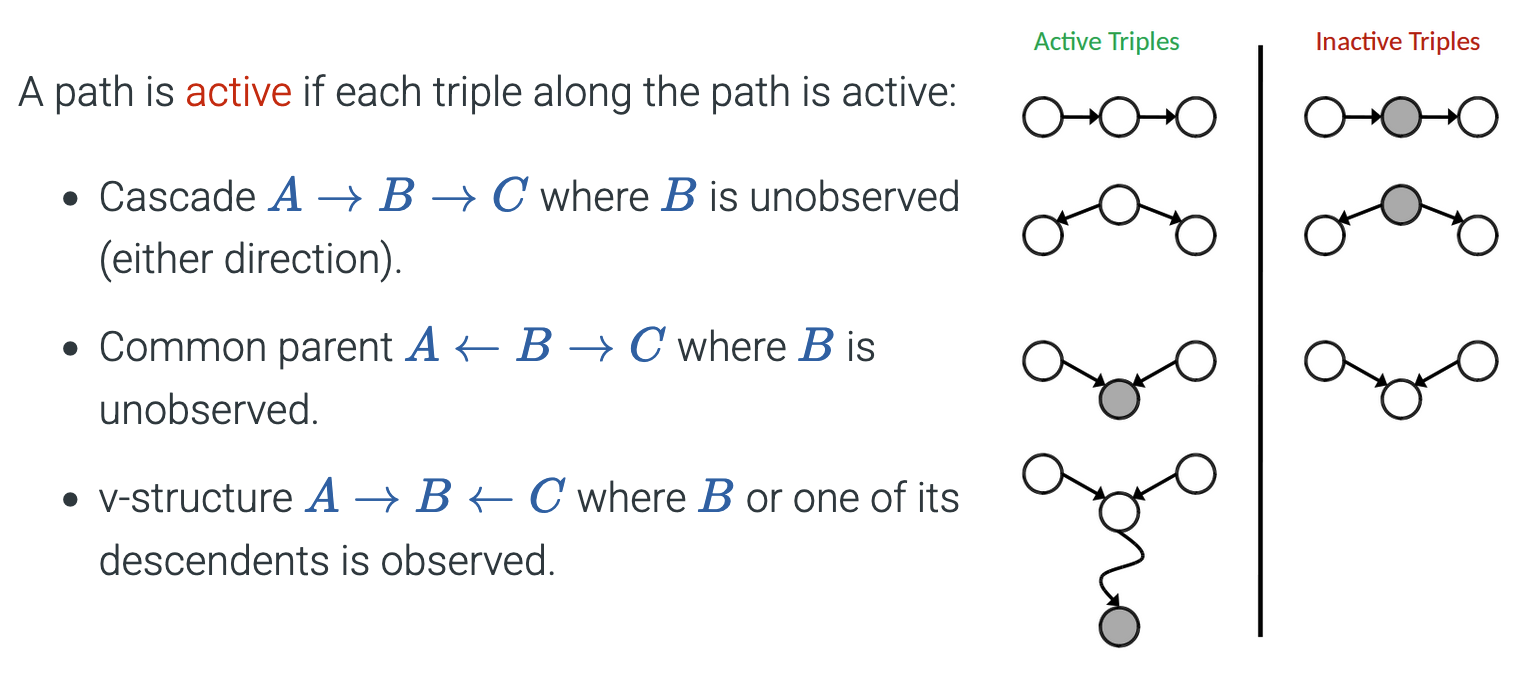
\includegraphics[width=.9\linewidth]{figures/triplets.png}
\end{figure}    

\newpage

\begin{thbox}{Cheat sheet for Gaussian models}
From the joint 
\[
p
\begin{pmatrix}
    \mathbf{x}\\
    \mathbf{y}
\end{pmatrix}
= \N
\begin{pmatrix}
    \begin{pmatrix}
        \mathbf{a}\\
        \mathbf{b}
    \end{pmatrix},
    \begin{pmatrix}
        \mathbf{A} & \mathbf{C}\\
        \mathbf{C^T} & \mathbf{B}
    \end{pmatrix}
\end{pmatrix},
\]
the marginal and conditional distributions are given by
\begin{align*}
    p(\mathbf{x}) &= \N(\mathbf{a}, \mathbf{A})\\
    p(\mathbf{y}) &= \N(\mathbf{b}, \mathbf{B})\\
    p(\mathbf{x \mid y}) &= \N(\mathbf{a + CB^{-1}(y - b)}, \mathbf{A - CB^{-1}C^T})\\
    p(\mathbf{y \mid x}) &= \N(\mathbf{b + C^T A^{-1}(x - a)}, \mathbf{B - C^T A^{-1}C}).
\end{align*}
On the other hand, from 
\begin{align*}
    p(\mathbf{x}) &= \N(\mathbf{m}, \mathbf{P})\\
    p(\mathbf{y \mid x}) &= \N(\mathbf{Hx + u}, \mathbf{R}),
\end{align*}
we can recover the joint distribution as
\[
p
\begin{pmatrix}
    \mathbf{x}\\
    \mathbf{y}
\end{pmatrix}
= \N
\begin{pmatrix}
    \begin{pmatrix}
        \mathbf{m}\\
        \mathbf{Hm + u}
    \end{pmatrix},
    \begin{pmatrix}
        \mathbf{P} & \mathbf{PH^T}\\
        \mathbf{HP} & \mathbf{HPH^T + R}
    \end{pmatrix}
\end{pmatrix},
\]
\end{thbox}
\textbf{In session exercises:} Ex. 1, Ex. 2
\newpage

\section{Nuclear power plant (AIMA, Ex 14.11)}

In your local nuclear power station, there is an alarm that senses when a temperature gauge exceeds a given threshold. The gauge measures the temperature of the core. Consider the Boolean variables $A$ (alarm sounds), $F_A$ (alarm is faulty), and $F_G$ (gauge is faulty) and the multi-valued nodes $G$ (gauge reading) and $T$ (actual core temperature).

\begin{enumerate}
    \item Draw a Bayesian network for this domain, given that the gauge is more likely to fail when the core temperature gets too high.

    \begin{solution}
        \begin{figure}[h]
            \centering
            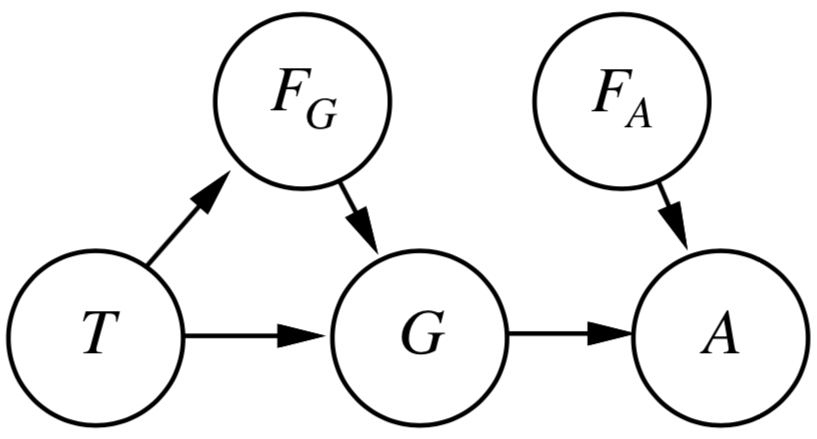
\includegraphics[width=0.4\textwidth]{figures/e3_nuclear.png}
        \end{figure}
    \end{solution}
    
    \item From your network topology, can you conclude $T \perp F_A \mid F_G$ and $T \perp F_A \mid F_G, A$?
    \begin{solution}

    All the path from $T$ to $F_A$ are ($T,F_G,G,A,F_A$) and ($T,G,A,F_A$).\\

    Knowing $F_G$, the triplet ($G, A, F_A$) is inactive (v-structure). Since it is present in both path, we can conclude that there are no active path, so $T \perp F_A \mid F_G$ is true.\\
    
    For the second relation, the triplet ($G, A, F_A$) becomes active as we observe $A$. The only way we can ensure conditional independence is by ensuring that at least one remaining triplet is inactive in each path.
    For the first path, we have ($T, F_G, G$) which is inactive (cascade) which makes the path inactive. However, for the second path, ($T, G, A$) is active (cascade) which makes the path active. We have at least one active path from $T$ to $F_A$ which prevents us to conclude the conditional independence in this case.
    \end{solution}
    \item Suppose there are just two possible actual and measured temperatures: low ($l$) and high ($h$). The probability that the gauge gives the correct temperature is $x$ when it is working, but $y$ when it is faulty. Give the conditional probability table associated with $G$.

    \begin{solution}
        The CPT for $G$ is shown below. Students should pay careful attention to the semantics of $F_G$, which is true when the gauge is faulty, \ie{} not working properly.
        \begin{table}[h!]
            \centering
            \begin{tabular}{cc|c}
                \toprule
                 $T$ & $F_G$ & $P(G = l | T, F_G)$ \\
                 \midrule
                 $l$ & 0 & $x$ \\
                 $l$ & 1 & $y$ \\
                 $h$ & 0 & $1 - x$ \\
                 $h$ & 1 & $1 - y$ \\
                 \bottomrule
            \end{tabular}
        \end{table}
    \end{solution}

    \item Suppose the alarm is always triggered by high measured temperatures, unless it is faulty, in which case it never sounds. Give the conditional probability table associated with $A$.

    \begin{solution}
        \begin{table}[h]
            \centering
            \begin{tabular}{cc|c}
                \toprule
                 $G$ & $F_A$ & $P(A = 1 | G, F_A)$ \\
                 \midrule
                 $l$ & 0 & 0 \\
                 $l$ & 1 & 0 \\
                 $h$ & 0 & 1 \\
                 $h$ & 1 & 0 \\
                 \bottomrule
            \end{tabular}
        \end{table}
    \end{solution}

    \item Suppose the gauge is not faulty and the alarm is triggered. Calculate an expression for the probability that the temperature of the core is too high, in terms of the various conditional probabilities in the network.

    \begin{solution}
        The probability of interest here is $P(T = h | A = 1, F_G = 0)$. Because the alarm's behavior is deterministic, we can deduce that $G$ indicates high ($h$). Hence, $P(T = h | A = 1, F_G = 0) = P(T = h | A = 1, G = h, F_G = 0)$. We also see that $A \perp T | G$. Therefore, we only need to calculate
        \begin{align*}
            P(T = h | G = h, F_G = 0) & = \frac{P(T = h, G = h, F_G = 0)}{P(G = h, F_G = 0)} \\
            & = \frac{P(G = h | T = h, F_G = 0) P(F_G = 0 | T = h) P(T = h)}{\sum_t P(G = h | t, F_G = 0) P(F_G = 0 | t) P(t)} ,
        \end{align*}
        which we cannot develop more as we don't know $P(T)$ and $P(F_G | T)$.
    \end{solution}
\end{enumerate}

\newpage

\section{Student--TA relationship}

The teaching assistant of the course is worried about the time he spends to prepare the exercise sessions. He wants to investigate the influence of students can have on his schedule. To do so, he builds the following model

\begin{figure}[h]
    \centering
    \begin{tikzpicture}[node distance = 2.5cm]
        \node[state] (S) {$S$};
        \node[state] (H) [right of=S] {$H$};

        \draw[arrow] (S) to (H);
    \end{tikzpicture}
\end{figure}

where $S$ is a r.v. denoting the number of students leaving the room between a theoretical lecture and the practical session that follows, and $H$ is a r.v. representing the number of hours spent to prepare the next session. He chooses the following relations for each variable
\begin{equation}
    \label{P_S}
    P(S = s) = \texttt{Poisson}(S=s;\lambda) = \dfrac{\lambda ^s e^{-\lambda}}{s!}
\end{equation}
\begin{equation}
    \label{P_H_g_S}
    H = \omega S + H_0 + \mathcal{N}(0, \var)
\end{equation}
where $H_0$ corresponds to the number of hours the TA should spend per session regarding its contract and $\omega$ is the influence weight of students over the TA.

\begin{enumerate}
    \item Identify the parameters of the Bayesian network and give the joint log-likelihood of one pair $(s_i, h_i)$ given the model.
    
    \begin{solution}
    Given the topology of the network, we have to identify $P(S=s)$ and $P(H = h \mid S = s)$. The former is given by~(\ref{P_S}) whereas the latter can be deduced from~(\ref{P_H_g_S}). We have 
    \begin{equation*}
        P(S = s) = \texttt{Poisson}(S=s;\lambda)
    \end{equation*}
    and
    \begin{equation*}
        P(H = h \mid S = s) = \mathcal{N}(\omega s + H_0, \var).
    \end{equation*}

    The parameters of those distributions are $\theta = [\lambda,   \omega,  \sigma]$.
    
    The likelihood of a pair $(s_i, h_i)$ can be derived from the network. We have 
    \begin{align*}
        P((s_i,h_i)\mid \theta) &= P(s_i)P(h_i \mid s_i)\\
        &= \dfrac{\lambda ^{s_i} e^{-\lambda}}{s_i!} \dfrac{1}{\sqrt{2\pi}\sigma}e^{-\frac{(h_i - \omega s_i - H_0)^2}{2\var}}
    \end{align*}
    from which we derive the log-likelihood
    \begin{equation}
        LL((s_i,h_i);\theta) = s_i \log{\lambda} - \lambda - \log{s_i!} - \log{\sqrt{2\pi}\sigma} - \dfrac{(h_i - \omega s_i - H_0)^2}{2\var}.
    \end{equation}
    \end{solution}
    \item The TA collects a set $\mathcal{D} = \{(s_i,h_i)\}_{i=1}^N$ of independent observations. Derive the maximum likelihood estimate of the parameters.

    \begin{solution}
        We first have to define the joint likelihood of those observations. Since they are assumed i.i.d., we have 
        $$
        P(\mathcal{D}\mid \theta) = \prod_{i=1}^N P((s_i,h_i)\mid \theta)
        $$
        Hence, deriving the log-likelihood
        \begin{align*}
        LL(\mathcal{D};\theta) &= \sum_i LL((s_i,h_i);\theta)\\
        &= -N(\lambda + \log{\sqrt{2\pi}\sigma}) + \sum_i s_i \log{\lambda} - \log{s_i!} - \dfrac{(h_i - \omega s_i - H_0)^2}{2\var}
        \end{align*}
        The maximum likelihood parameters can be found by cancelling the derivative of the log-likelihood w.r.t. each parameter.
        
        For $\lambda$ we have
        \begin{align*}
            \dfrac{\partial LL}{\partial \lambda} &= -N + \sum_i \dfrac{s_i}{\lambda}\\
            &= 0
        \end{align*}
        which gives $\boxed{\lambda_{\text{MLE}} = \dfrac{1}{N}\sum_i s_i}$. 

        For $\sigma$ we have
        \begin{align*}
            \dfrac{\partial LL}{\partial \sigma} &= -\dfrac{1}{\sigma}\bigg(N -\sum_i \dfrac{(h_i - \omega s_i - H_0)^2}{\var}\bigg)\\
            &\propto N -\dfrac{1}{\var}\sum_i (h_i - \omega s_i - H_0)^2\\
            &= 0
        \end{align*}
        which gives $\boxed{\var_{\text{MLE}} = \dfrac{1}{N}\sum_i (h_i - \omega s_i - H_0)^2}$.

        For $\omega$ we have
        \begin{align*}
            \dfrac{\partial LL}{\partial \omega} &= \sum_i \dfrac{s_i(h_i - \omega s_i - H_0)}{\var}\\
            &\propto \bigg(\sum_i s_i(h_i - H_0)\bigg) - \omega\sum_i s_i^2\\
            &= 0
        \end{align*}
        which gives $\boxed{\omega_{\text{MLE}} = \dfrac{\sum_i s_i(h_i - H_0)}{\sum_i s_i^2}}$.
        
    \end{solution} 
    \item The TA has just started to collect observations of students leaving the classroom. Being an adept of the Bayes' school, he knows that using MLE can lead to overfitting. Hence, he decides to incorporate uncertainty in his analysis of the parameter $\lambda$ as he has no strong knowledge about it. Using a prior $\lambda \sim \texttt{Gamma}(\alpha, \beta)$, what would be the posterior distribution $P(\lambda \mid \mathcal{S} = \{s_i\}_{i=1}^N)$?\\
    
    \textit{Hint:} $\texttt{Gamma}(x \mid \alpha, \beta) = \frac{1}{Z}x^{\alpha - 1} e^{-\beta x}$, with $Z$ a normalizing constant.
    
    \begin{solution}
        Using the Bayes' theorem
        \begin{align*}
            P(\lambda \mid \mathcal{S}) &\propto P(\mathcal{S} \mid \lambda) P(\lambda)\\
            &\propto \lambda^{\alpha - 1} e^{-\beta \lambda} \prod_i \dfrac{\lambda ^{s_i} e^{-\lambda}}{s_i!}\\
            &= \lambda^{\alpha - 1} e^{-\beta \lambda} \bigg(\dfrac{\lambda ^{\sum_i s_i} e^{-N\lambda}}{\prod_is_i!}\bigg)\\
            &\propto \lambda^{(\alpha + \sum_i s_i - 1)} e^{-(\beta + N) \lambda}
        \end{align*}
        which corresponds to $\texttt{Gamma}(\alpha + \sum_i s_i,\  \beta + N)$, the posterior density. Note that $\propto$ stands for the normalizing constant of the posterior density. Everything that does not depends explicitly on the parameter $\lambda$ can be absorbed in the constant if it multiplies the whole.
    \end{solution}
    \item Knowing that the mean, the variance and the mode of $\texttt{Gamma}(\alpha, \beta)$ are respectively $\dfrac{\alpha}{\beta}$, $\dfrac{\alpha}{\beta^2}$ and $\dfrac{\alpha-1}{\beta}$, interpret how they evolve w.r.t. $N$ between the prior and the posterior.

    \begin{solution}
        We have 
        $$\E(\lambda): \dfrac{\alpha}{\beta} \Rightarrow \dfrac{\alpha + \sum_i s_i}{\beta + N},$$
        $$\V(\lambda): \dfrac{\alpha}{\beta^2} \Rightarrow \dfrac{\alpha + \sum_i s_i}{(\beta + N)^2}$$
        and
        $$\underset{\lambda}{\arg \max}P(\lambda\mid .): \dfrac{\alpha -1}{\beta} \Rightarrow \dfrac{\alpha + \sum_i s_i - 1}{\beta + N}.$$
        When $N = 0$, the prior and the posterior are similar, which is expected. When $N \rightarrow \infty$, knowing that $s\in \mathbb{N}$ by definition (number of students leaving the room), we can assume that, for reasonable values of $\alpha, \beta$, we have $\sum_i s_i \gg \alpha$ and $N \gg \beta$. This implies that the mean and the mode converge to the same value corresponding to $\lambda_{\text{MLE}}$. The variance decreases towards 0, which suggests that $\lambda_{\text{MLE}}$ is the best and unique estimate of $\lambda$ for an infinite amount of observations. This illustrates the trade-off between likelihood and prior in a Bayesian parameter learning setting. As more data are observed, the uncertainty about a parameter decreases smoothly from the prior to the likelihood.
    \end{solution}
\end{enumerate}

\newpage

\section{Car diagnosis (AIMA, Ex 14.8)}

Let be the following Bayesian network describing some features of a car's electrical system and engine. Each variable is Boolean, and the true value indicates that the corresponding aspect of the vehicle is in working order.

\begin{figure}[h]
    \centering
    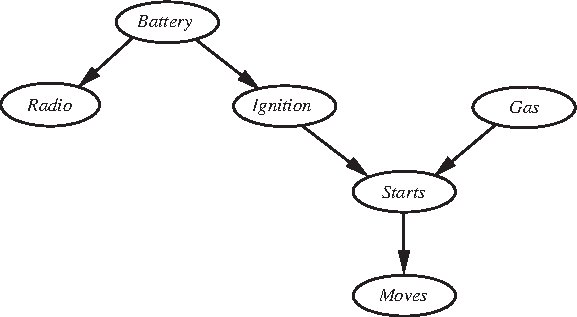
\includegraphics[width=0.6\textwidth]{figures/e3_car.pdf}
\end{figure}

\begin{enumerate}
    \item Extend the network with the Boolean variables IcyWeather and StarterMotor.

    \begin{solution}
        IcyWeather is not caused by any of the car-related variables, so needs no parents. It directly affects the battery and the starter motor. StarterMotor is an additional precondition for Starts.

        \begin{figure}[h]
            \centering
            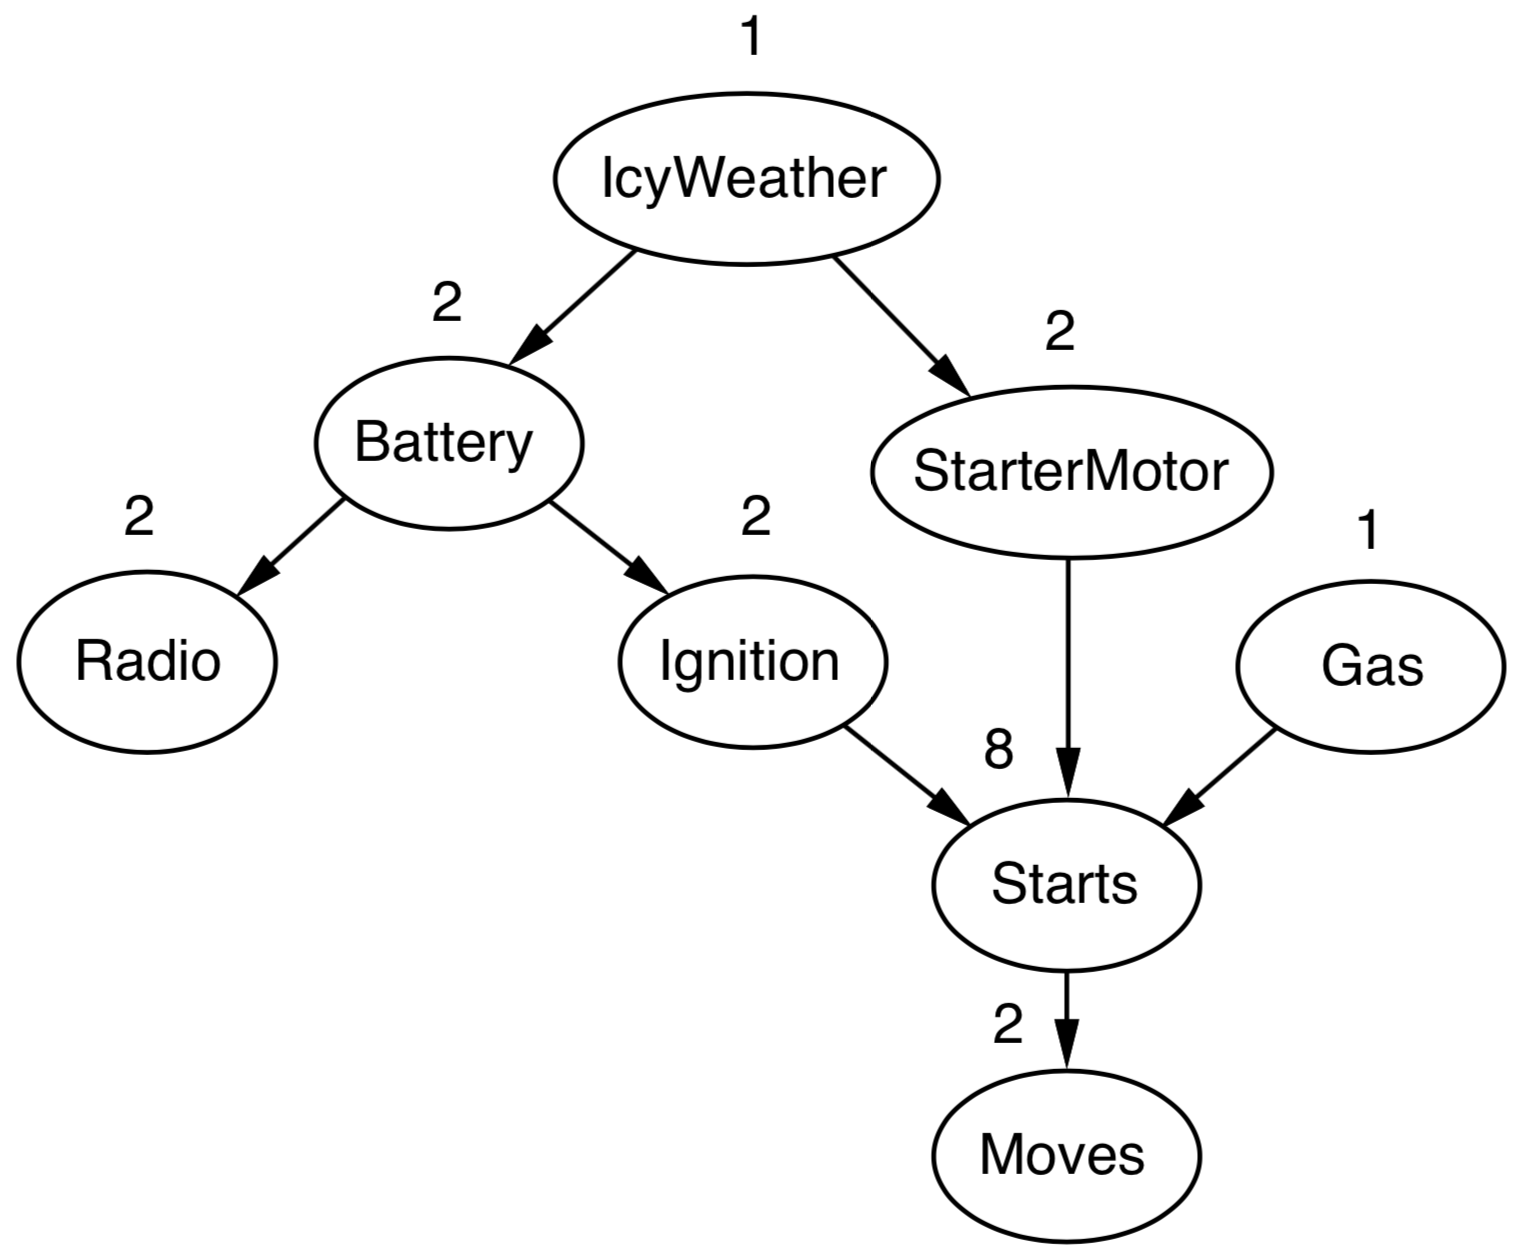
\includegraphics[width=0.6\textwidth]{figures/e3_car_full.png}
        \end{figure}
    \end{solution}

    \item According to your knowledge of cars, give reasonable conditional probability tables for all the nodes.

    \begin{solution}
        Reasonable probabilities may vary a lot depending on the kind of car and perhaps the personal experience of the assessor. The following values indicate the general order of magnitude and relative values that would be reasonable:
        \begin{itemize}
            \item A reasonable prior for IcyWeather might be $0.05$ (depending on location and season).
            \item $P(Battery|IcyWeather)=0.95,P(Battery|\lnot IcyWeather)=0.997$.
            \item $P(StarterMotor|IcyWeather) = 0.98$, $P(Battery|\lnot IcyWeather) = 0.999$.
            \item $P(Radio|Battery) = 0.9999, P (Radio|\lnot Battery) = 0.05$.
            \item $P(Ignition|Battery) = 0.998, P (Ignition|\lnot Battery) = 0.01$.
            \item $P(Gas) = 0.995$.
            \item $P(Starts|Ignition,StarterMotor,Gas) = 0.9999$, other entries $0.0$.
            \item $P(Moves|Starts) = 0.998$.
        \end{itemize}
    \end{solution}

    \item How many independent values are contained in the joint probability distribution for eight Boolean nodes, assuming that no conditional independence relations are known to hold among them?

    \begin{solution}
        With 8 Boolean variables, the joint has $2^8 - 1 = 255$ independent entries.
    \end{solution}

    \item How many independent probability values do your network tables contain?

    \begin{solution}
        Given the topology with IcyWeather and StarterMotor, the total number of independent CPT entries is $1 + 2 + 2 + 2 + 2 + 1 + 8 + 2 = 20$.
    \end{solution}
\end{enumerate}

\newpage

\section{Gaussian parameter learning with known $\var$}
You have in your possession a high-tech laser that emits light of intensity $\mu_l$ with great precision. You want to use it to test a new light-intensity measurement device. You assume that your measures $y_i$ follow a Gaussian distribution $\N(\mu_y,\var)$ with $\mu_y \sim \N(\mu_l, \sigma_l^2)$ corresponding to the model of your laser given in the manual. You assume that $\var$ is fixed and that you can determine it.

You have access to $\mathcal{Y}_c$ a calibration set of $C$ observations and you want to make $N$ new measures with your device. You want to study how you can reduce your uncertainty about the measures using $\mathcal{Y}_c$.

\begin{enumerate}
    \item Compute the prior and posterior predictive distributions $P(y)$ and $P(y\mid \mathcal{Y}_c)$ if you have access to one observation, i.e. $\mathcal{Y}_c = \{y_o\}$.
    
    \begin{solution}
        The following exercise uses the Gaussian model identities (cfr. theoretical reminder of this session).\\

        We first identify the components we have:
        \begin{itemize}
            \item $P(y\mid \mu_y) = \N(\mu_y,\var)$
            \item $P(\mu_y) = \N(\mu_l,\sigma_l^2)$
        \end{itemize}
        \textbf{Prior predictive}\\
        $$P(y) = \int P(y\mid \mu_y) P(\mu_y) d\mu_y.$$
        From Gaussian identities, you can identify different parameters as follows
        \begin{align*}
            \mathbf{x} &= \mu_y\\
            \mathbf{m} &= \mu_l\\
            \mathbf{P} &= \sigma_l^2\\
            \mathbf{y} &= y\\
            \mathbf{H} &= 1\\
            \mathbf{u} &= 0\\
            \mathbf{R} &= \var
      \end{align*}
      which corresponds to the joint
      $$
      P(\mu_y, y) = \N
      \begin{pmatrix}
        \begin{pmatrix}
            \mu_l\\
            \mu_l\\
        \end{pmatrix},
        \begin{pmatrix}
            \sigma_l^2 & \sigma_l^2\\
            \sigma_l^2 & \sigma_l^2 + \var\\
        \end{pmatrix}
    \end{pmatrix}
      $$
      from which we extract $P(y) = \N(\mu_l, \var + \sigma_l^2)$.

      \textbf{Posterior predictive}\\
      $$P(y\mid \mathcal{Y}_c) = \int P(y\mid \mu_y) P(\mu_y \mid \mathcal{Y}_c) d\mu_y.$$
      
      We first have to identify the posterior $P(\mu_y \mid \mathcal{Y}_c)$.
      Once again, from Gaussian identities, knowing $P(\mathcal{Y}_c \mid \mu_y)$ and $P(\mu_y)$ you can identify different parameters as follows
        \begin{align*}
            \mathbf{x} &= \mu_y\\
            \mathbf{m} &= \mu_l\\
            \mathbf{P} &= \sigma_l^2\\
            \mathbf{y} &= y_o\\
            \mathbf{H} &= 1\\
            \mathbf{u} &= 0\\
            \mathbf{R} &= \var
      \end{align*}
      which corresponds to the joint
      $$
      P(\mu_y, y_o) = \N
      \begin{pmatrix}
        \begin{pmatrix}
            \mu_l\\
            \mu_l\\
        \end{pmatrix},
        \begin{pmatrix}
            \sigma_l^2 & \sigma_l^2\\
            \sigma_l^2 & \sigma_l^2 + \var\\
        \end{pmatrix}
    \end{pmatrix}
      $$
      from which we extract 
      \begin{align*}
      P(\mu_y \mid y_o) &= \N(\mu_{post}, \sigma_{post}^2)\\ 
                    &= \N\bigg(\mu_l + \dfrac{\sigma_l^2}{\var + \sigma_l^2}(y_o - \mu_l), \sigma_l^2 - \dfrac{\sigma_l^4}{\var + \sigma_l^2}\bigg).
      \end{align*}
      After simplification, we identify the posterior parameters as 
      $$\mu_{post} = \dfrac{\var}{\var + \sigma_l^2}\mu_l + \dfrac{\sigma_l^2}{\var + \sigma_l^2}y_o$$
      and
      $$\sigma_{post}^2 = \dfrac{\var}{\sigma_l^2 + \var} \sigma_l^2.$$
%       We derive
%       \begin{align*}
%           P(\mu_y \mid \mathcal{Y}_c) &\propto P(\mathcal{Y}_c \mid \mu_y)P(\mu_y)\\
%           &\propto e^{-\frac{(\mu_y - \mu_l)^2}{2\sigma_l^2}}\prod_{i=1}^C e^{-\frac{(y_i - \mu_y)^2}{2\var}}\\
%           &= e^{-\frac{(\mu_y - \mu_l)^2}{2\sigma_l^2} -\frac{\sum_i(y_i - \mu_y)^2}{2\var}}
%       \end{align*}
%       looking at the exponent
%       \begin{align*}
%           -\frac{(\mu_y - \mu_l)^2}{2\sigma_l^2} -\frac{\sum_i(y_i - \mu_y)^2}{2\var} &= -\frac{1}{2}\bigg( \frac{\mu_y^2}{\sigma_l^2} + \frac{\mu_l^2}{\sigma_l^2} - \frac{2\mu_y\mu_l}{\sigma_l^2} + \frac{C\mu_y^2}{\var} + \frac{\sum_i y_i^2}{\var} - \frac{2\sum_i y_i\mu_y}{\var}\bigg)
%       \end{align*}
%       we can get rid of all elements not depending on $\mu_y$ as they will be absorbed in the normalizing constant when taking to the exponent. Furthermore, if we set $C\mu_{MLE}= C\bar{y} = \sum_i y_i$, the reduced exponent becomes
%       \begin{align*}
%           \text{exponent} &= -\frac{1}{2}\bigg( \frac{\mu_y^2}{\sigma_l^2} - \frac{2\mu_y\mu_l}{\sigma_l^2} + \frac{C\mu_y^2}{\var} - \frac{2C \bar{y}\mu_y}{\var}\bigg)\\
%           &= -\frac{1}{2}\bigg[ \mu_y^2\bigg(\frac{1}{\sigma_l^2} + \frac{C}{\var}\bigg) - 2\mu_y\bigg(\frac{\mu_l}{\sigma_l^2} + \frac{C\bar{y}}{\var}\bigg)\bigg]\\
%           &= -\frac{1}{2}\bigg(\frac{1}{\sigma_l^2} + \frac{C}{\var}\bigg)\bigg[\mu_y^2 - 2\mu_y\dfrac{\bigg(\frac{\mu_l}{\sigma_l^2} + \frac{C\bar{y}}{\var}\bigg)}{\bigg(\frac{1}{\sigma_l^2} + \frac{C}{\var}\bigg)}\bigg]\\
%       \end{align*}
%     we can add $\frac{\bigg(\frac{\mu_l}{\sigma_l^2} + \frac{C\bar{y}}{\var}\bigg)^2}{\bigg(\frac{1}{\sigma_l^2} + \frac{C}{\var}\bigg)^2} - \frac{\bigg(\frac{\mu_l}{\sigma_l^2} + \frac{C\bar{y}}{\var}\bigg)^2}{\bigg(\frac{1}{\sigma_l^2} + \frac{C}{\var}\bigg)^2}$ into the brackets to complete the square. However, we observe that this element does not depends on $\mu_y$. Hence, we use the addition to complete the square and the substraction is absorbed in the normalizing constant. We are left with 
%     \begin{align*}
%           \text{exponent} &= -\frac{1}{2}\bigg(\frac{1}{\sigma_l^2} + \frac{C}{\var}\bigg)\bigg[\mu_y - \dfrac{\bigg(\frac{\mu_l}{\sigma_l^2} + \frac{C\bar{y}}{\var}\bigg)}{\bigg(\frac{1}{\sigma_l^2} + \frac{C}{\var}\bigg)}\bigg]^2
%    \end{align*}
%     which gives $$\mu_{post} = \dfrac{\mu_l\var + C\bar{y}\sigma_l^2}{\var + C\sigma_l^2} = \dfrac{\var}{\var + C\sigma_l^2}\mu_l + \dfrac{C\sigma_l^2}{\var + C\sigma_l^2}\mu_{MLE}$$ 
%     and 
%     $$\sigma_{post}^2 = \bigg(\dfrac{1}{\sigma_l^2} + \dfrac{C}{\var}\bigg)^{-1} = \dfrac{\var}{C\sigma_l^2 + \var} \sigma_l^2.$$

    Following the same development as for the prior predictive, we have 
    $$P(y\mid \mathcal{Y}_c) = \N(\mu_{post}, \var + \sigma_{post}^2).$$
    \end{solution}
    \item Looking at you predictive uncertainty, what is the benefit of incorporating $\mathcal{Y}_c$?
    
    \begin{solution}
        As a reminder, we found
        $$P(y) = \N(\mu_l, \var + \sigma_l^2).$$
        $$P(y\mid \mathcal{Y}_c) = \N(\mu_{post}, \var + \sigma_{post}^2).$$
        Comparing only the variances, we have
        \begin{align*}
            \var + \sigma_l^2 &\overset{?}{\lessgtr} \var + \sigma_{post}^2\\
            \sigma_l^2 &\overset{?}{\lessgtr} \sigma_{post}^2\\
            1 &\overset{?}{\lessgtr} \dfrac{\var}{\sigma_l^2 + \var}\\
            \sigma_l^2 &\geq 0
        \end{align*}
        and we deduce that the posterior predictive has a smaller or equal variance to the prior one. We conclude that incorporating the calibration set can reduce uncertainty about the measures.\\

        If we computed the variance for a calibration set of $C$ observations, we would have found a posterior variance
        $$\sigma_{post}^2 = \dfrac{\var}{C\sigma_l^2 + \var} \sigma_l^2.$$
        Since $\var$ is fixed, we see that including more observations reduces even more the posterior predictive variance. In the limit case $C\to \infty$, the posterior predictive variance converges to $\var$ which corresponds to the uncertainty
        of the instrument (you can't reach a lower uncertainty, it is called the aleatoric uncertainty). 
        
    \end{solution}
\end{enumerate}

\newpage

\section{Independence}

\begin{figure}[h]
    \centering
    \begin{tikzpicture}[node distance = 2.5cm]
        \node[state] (A) {$A$};
        \node[state] (B) [below of=A] {$B$};
        \node[state] (C) [right of=B] {$C$};
        \node[state] (D) [below of=B] {$D$};
        \node[state] (E) [below right of=C] {$E$};
        \node[state] (F) [left of=B] {$F$};

        \draw[arrow] (A) to (B);
        \draw[arrow] (A) to (C);
        \draw[arrow] (B) to (D);
        \draw[arrow] (C) to (D);
        \draw[arrow] (C) to (E);
        \draw[arrow] (A) to (F);
        \draw[arrow] (B) to (F);
    \end{tikzpicture}
\end{figure}

Considering the hereabove Bayesian network, which of the following statements are enforced by the network structure?

\begin{solution}
    We apply the d-separation algorithm. To show that two variables $X$ and $Y$ could be dependent, it is sufficient to find a single \emph{active} (undirected) path from $X$ to $Y$. A path is active if all of its consecutive triplets are active.
\end{solution}

\begin{enumerate}
    \item $P(B, C) = P(B) P(C)$

    \begin{solution}
        This is true iff (if and only if) $B \perp C$ ($B$ is independent from $C$). The three paths that link $B$ and $C$ are $(B, A, C)$, $(B, D, C)$ and $(B, F, A, C)$. $(B, A, C)$ is active because $A$ is unknown ($\wedge$-structure). We cannot guarantee that $B \perp C$.
    \end{solution}

    \item $P(B, C | A) = P(B | A) P(C | A)$

    \begin{solution}
        This is true iff $B \perp C | A$. This time, $(B, A, C)$ is not active because $A$ is known. $(B, D, C)$ is not active either because $D$ is unknown ($\vee$-structure). In $(B, F, A, C)$, the triplet $(B, F, A)$ is active, but $(F, A, C)$ is not. We can guarantee that $B \perp C | A$.
    \end{solution}

    \item $P(F, E) = P(F) P(E)$

    \begin{solution}
        This is true iff $F \perp E$. The four paths that link $F$ and $E$ are $(F, A, C, E)$, $(F, A, B, D, C, E)$, $(F, B, A, C, E)$ and $(F, B, D, C, E)$. In $(F, A, C, E)$, the triplets $(F, A, C)$ ($\wedge$-structure) and $(A, C, E)$ are both active. We cannot guarantee that $F \perp E$.
    \end{solution}

    \item $P(F | A, D, E) = P(F | A, D)$

    \begin{solution}
        This is true iff $F \perp E | A, D$. This time, the triplets $(F, A, C)$, $(F, A, B)$ and $(B, A, C)$ are inactive ($\wedge$-structure, but $A$ is known). In $(F, B, D, C, E)$, $(F, B, D)$ is active. Indeed, knowing an extremity of a triplet does not impact whether it is active or not. Only the center variable is important. Then we have $(B, D, C)$ which is active ($\vee$-structure, but $D$ is known) and $(D, C, E)$ also. Hence, $(F, B, D, C, E)$ is active and we cannot guarantee that $F \perp E | A, D$.
    \end{solution}

    \item $P(B, E) = \sum_{a, c, d, f} P(a) P(B | a) P(c | a) P(d | B, c) P(E | c) P(f | a, B)$

    \begin{solution}
        We notice that
        \begin{equation*}
            P(A, B, C, D, E, F) = P(A) P(B | A) P(C | A) P(D | B, C) P(E | C) P(F | A, B)
        \end{equation*}
        corresponds exactly to
        \begin{equation*}
            P(X_1, \dots, X_n) = \prod_{i = 1}^n P(X_i | parents(X_i)) ,
        \end{equation*}
        for the considered network, which we know is guaranteed. We also known that
        \begin{equation*}
            P(B, E) = \sum_{a, c, d, f} P(a, B, c, d, E, f)
        \end{equation*}
        Hence, the initial statement is always true.
    \end{solution}
\end{enumerate}

For the same network, use inference by variable elimination to compute $P(E | A = 1, B = 1)$.

\begin{solution}
    We have
    \begin{align*}
        P(E | A = 1, B = 1) & = \alpha \sum_{c, d} P(A = 1, B = 1, c, d, E)\\
        & = \alpha \sum_{c, d} P(A = 1) P(B = 1| A = 1) P(c| A = 1) P(d|B = 1, c) P(E|c) \\
        & = \alpha P(A = 1) P(B = 1 | A = 1) \sum_{c} P(c|A = 1) P(E|c)\sum_d P(d|B = 1,c) .
    \end{align*}
    We define the initial factors as
    \begin{align*}
        f_1 & = P(A=1) \\
        f_2 & = P(B=1 | A=1) \\
        f_3(C) & = P(C|A=1) \\
        f_4(E, C) & = P(E|C) \\
        f_5(C, D) & = P(D|B=1, C)
    \end{align*}
    and the composite factors as
    \begin{align*}
        f_6(C) & = \sum_d f_5(C, d) \\
        f_7(C, E) & = f_3(C) \times f_4(E, C) \times f_6(C) \\
        f_8(E) & = \sum_c f_7(c, E) \\
        f_9(E) & = f_1 \times f_2 \times f_7(E) .
    \end{align*}
    Finally,
    \begin{equation*}
        P(E | A = 1, B = 1) = \alpha f_9(E) = \frac{f_9(E)}{\sum_e f_9(e)}.
    \end{equation*}
\end{solution}

\newpage

\section{Pacbaby (UC Berkeley CS188, Spring 2014)}

Pacman and Pacwoman have been searching for each other in the maze. Pacwoman has been pregnant with a baby, and just this morning she has given birth to Pacbaby\footnote{Congratulations!}. Because Pacbaby was born before Pacman and Pacwoman were reunited in the maze, he has never met his father. Naturally, Pacwoman wants to teach Pacbaby to recognize his father, using a set of pictures of Pacman. She also has several pictures of ghosts to use as negative examples.

\begin{figure}[h]
    \centering
    
\includegraphics[width=0.5\textwidth]{figures/e5_pacbaby.jpg}
\end{figure}

Because the pictures are black and white, and were taken from various angles, Pacwoman has decided to teach Pacbaby to identify Pacman based on salient features: the presence of a bowtie $B$, hat $H$ or mustache $M$. The following table summarizes the content of the pictures. Each feature takes realization in $\cbk{0, 1}$, where $0$ and $1$ mean the feature is respectively absent and present. The subject of the picture is described by a random variable $S \in \cbk{0, 1}$, where $0$ is a ghost and $1$ is Pacman.

\begin{table}[h]
    \centering
    \begin{tabular}{ccc|c}
        \toprule
        $B$ & $H$ & $M$ & $S$ \\
        \midrule
        0 & 0 & 0 & 1 \\
        1 & 0 & 0 & 0 \\
        1 & 0 & 1 & 1 \\
        1 & 1 & 0 & 0 \\
        0 & 1 & 0 & 0 \\
        1 & 1 & 1 & 1 \\
        \bottomrule
    \end{tabular}
\end{table}

\begin{enumerate}
    \item Suppose Pacbaby has a Naive Bayes based brain. Draw the Bayesian network that would represent the dependencies between $S$, $B$, $H$ and $M$ for Pacbaby.

    \begin{solution}
        \begin{figure}[H]
            \centering
            \begin{tikzpicture}[node distance = 2cm]
                \node[state] (S) {$S$};
                \node[state] (B) [below left of=S] {$B$};
                \node[state] (H) [below of=S] {$H$};
                \node[state] (M) [below right of=S] {$M$};

                \draw[arrow] (S) to (B);
                \draw[arrow] (S) to (H);
                \draw[arrow] (S) to (M);
            \end{tikzpicture}
        \end{figure}
    \end{solution}

    \item Write the Bayesian classification rule for this problem, \ie{} the formula that given a data point $(b, h, m)$ returns the most likely subject. Write the formula in terms of conditional and prior probabilities. What does the formula become under the assumptions of Pacbaby ?

    \begin{solution}
        Given $(b, h, m)$, the most likely subject is given by the \emph{maximum a posteriori} (MAP) estimation
        \begin{align*}
            s_{\text{MAP}} & = \arg\max_{s} P(s | b, h, m) \\
            & = \arg\max_{s} P(b, h, m | s) P(s) .
        \end{align*}
        Under the naive Bayes assumptions of Pacbaby, $B$, $H$ and $M$ become independent conditionally to $S$, \ie{} $P(B, H, M | S) = P(B | S) P(H | S) P(M | S)$. Then, the formula becomes
        \begin{align*}
            s_{\text{MAP}} & = \arg\max_{s} P(b | s) P(h | s) P(m | s) P(s) .
        \end{align*}
    \end{solution}

    \item What are the parameters of this model? Give estimates of these parameters according to the pictures provided by Pacwoman.

    \begin{solution}
        The parameters of the model are the elements of the prior vector $P(S)$ and the (conditional) probability matrices $P(B | S)$, $P(H | S)$ and $P(M | S)$. An (unbiased) estimation of these elements can be computed as the frequency of their respective events within the learning set (of pictures).

        \begin{table}[h]
            \centering
            \begin{tabular}{c|cccc}
                \toprule
                $S$ & $P(S)$ & $P(B = 1 | S)$ & $P(H = 1 | S)$ & $P(M = 1 | S)$ \\
                \midrule
                0 & $\frac{3}{6}$ & $\frac{2}{3}$ & $\frac{2}{3}$ & $\frac{0}{3}$ \\
                1 & $\frac{3}{6}$ & $\frac{2}{3}$ & $\frac{1}{3}$ & $\frac{2}{3}$ \\
                \bottomrule
            \end{tabular}
        \end{table}
    \end{solution}

    \item Pacman eventually shows up wearing a bowtie, but no hat or mustache. Will Pacbaby recognize his father?

    \begin{solution}
        Pacbaby will recognize his father if $s_{\text{MAP}} = 1$ for $(b, h, m) = (1, 0, 0)$. Using the parameters estimated previously, we have
        \begin{align*}
            P(b | 0) P(h | 0) P(m | 0) P(0) & = \frac{2}{3} \times \rbk*{1 - \frac{2}{3}} \times \rbk*{1 - \frac{0}{3}} \times \frac{3}{6} \approx \num{0.111} \\
            P(b | 1) P(h | 1) P(m | 1) P(1) & = \frac{2}{3} \times \rbk*{1 - \frac{1}{3}} \times \rbk*{1 - \frac{2}{3}} \times \frac{3}{6} \approx \num{0.074} .
        \end{align*}
        Therefore, $s_{\text{MAP}} = 0$, meaning that Pacbaby will \emph{not} recognize his father.
    \end{solution}
\end{enumerate}

\newpage

\section{Predict your grade}

\begin{figure}[h]
    \centering
    \begin{tikzpicture}[node distance = 2cm]
        \node[state] (X1) {$x_1$};
        \node[state] (X2) [right of=X1] {$x_2$};
        \node[state] (X3) [right of=X2] {$x_3$};
        \node[state] (Y) [below of=X2] {$y$};

        \draw[arrow] (X1) to (X2);
        \draw[arrow] (X2) to (X3);
        \draw[arrow] (X1) to (Y);
        \draw[arrow] (X2) to (Y);
        \draw[arrow] (X3) to (Y);
    \end{tikzpicture}
\end{figure}

The hereabove Bayesian network represents how the final grade of a class is computed. In this model, $x_1$, $x_2$ and $x_3$ respectively denote the grades obtained by a student at the homework, project and exam. The teaching assistant that grades the homework also grades the project and the exam, which introduces a slight bias in the corrections. In particular, $x_2 \sim \N(a_1 x_1 + \mu_2, \sigma_2^2)$ and $x_3 \sim \N(a_2 x_2 + \mu_3, \sigma_3^2)$. Finally, $y \sim \N(a_3 x_1 + a_4 x_2 + a_5 x_3 + \mu_y, \sigma_y^2)$ stands for the final grade, which is a linear combination of the grades obtained by the student during the semester plus some Gaussian noise due to rounding errors. Answer the following questions about this model.

\begin{enumerate}
    \item Assuming the parameters of the model are known, what is the expected value of $y$ given $x_1$ and $x_2$.

    \begin{solution}
        Our task is to find the expectation
        \begin{equation*}
            \underset{p(y | x_1, x_2)}{\E} \sbk{y} = \int y \, p(y | x_1, x_2) \d{y} .
        \end{equation*}
        We know that
        \begin{equation*}
            p(y | x_1, x_2) = \int p(y | x_1, x_2, x_3) \, p(x_3 | x_1, x_2) \d{x_3} ,
        \end{equation*}
        where $p(y | x_1, x_2, x_3)$ and $p(x_3 | x_1, x_2)$ are linear Gaussian distributions given in the statement. Therefore, we have
        \begin{equation*}
            p(y | x_1, x_2) = \N\rbk*{a_3 x_1 + a_4 x_2 + a_5 (a_2 x_2 + \mu_3) + \mu_y, (a_5 \sigma_3)^2 + \sigma_y^2}
        \end{equation*}
        and, by definition of a Gaussian distribution,
        \begin{equation*}
            \underset{p(y | x_1, x_2)}{\E} \sbk{y} = a_3 x_1 + (a_4 + a_5 a_2) x_2 + a_5 \mu_3 + \mu_y.
        \end{equation*}
    \end{solution}

    \item Suppose now that the model's parameters are unknown. Given a learning set $d = \cbk{(x_{i,1}, x_{i,2}, y_i)}$ of $N$ independent and identically distributed points, determine the model that best describes $d$.

    \begin{solution}
        We know that the distribution of $y$ given $x_1$ and $x_2$ takes the form $\N(w_1 x_1 + w_2 x_2 + b, \sigma^2)$. Then, our task is to find the parameters $h = (w_1, w_2, b, \sigma)$ that maximize the likelihood of $d$, \ie{} the \emph{maximum likelihood estimation} (MLE)
        \begin{align*}
            h_{\text{MLE}} & = \arg \max_w p(d | h) \\
            & = \arg \max_h \prod_i p(x_i, y_i | h) \\
            & = \arg \max_h \log \prod_i p(x_i, y_i | h) \\ \displaybreak
            & = \arg \max_h \sum_i \log p(x_i, y_i | h) \\
            & = \arg \max_h \sum_i \log p(y_i | h, x_i) + \log p(x_i) \\
            & = \arg \max_h \sum_i \log p(y_i | h, x_i) \\
            & = \arg \max_h \sum_i \log \sbk*{\frac{1}{\sqrt{2 \pi \sigma^2}} \exp\rbk*{- \frac{(w^T x_i - y_i)^2}{2 \sigma^2}}} \\
            & = \arg \max_h \sum_i - \frac{1}{2} \log (2 \pi \sigma^2) - \frac{(w^T x_i - y_i)^2}{2 \sigma^2} \\
            & = \arg \min_h \log \sigma^2 + \frac{1}{\sigma^2} \frac{1}{N} \sum_i (w^T x_i - y_i)^2 ,
        \end{align*}
        where $x_i = \mat{x_{i,1} & x_{i,2} & 1}^T$ and $w = \mat{w_1 & w_2 & b}^T$. In the last expression, we observe that the summation term is independent from $\sigma$. Therefore,
        \begin{align*}
            w_{\text{MLE}} & = \arg \min_w \sum_i (w^T x_i - y_i)^2 ,
        \end{align*}
        which exactly corresponds to a \emph{linear regression} problem. Then, we find $w_{\text{MLE}}$ by canceling the gradient with respect to $w$, \ie{}
        \begin{align*}
            0 & = \nabla_{\!w} \sum_i (w^T x_i - y_i)^2 \\
            & = \nabla_{\!w} \sum_i (w^T x_i - y_i) (w^T x_i - y_i) \\
            & = \nabla_{\!w} \sum_i (w^T x_i)^2 + y_i^2 - 2 w^T x_i y_i \\
            & = \nabla_{\!w} \rbk*{w^T X^T X w + Y^T Y - 2 w^T X^T Y} \\
            & = 2 X^T X w - 2 X^T Y
        \end{align*}
        where $X = (x_i^T) \in \R^{N \times 3}$ and $Y = (y_i) \in \R^{N}$. Finally, we have
        \begin{alignat*}{2}
            && 0 & = X^T X w_{\text{MLE}} - X^T Y \\
            \Leftrightarrow \quad && w_{\text{MLE}} & = (X^T X)^{-1} X^T Y .
        \end{alignat*}
        Afterwards, we find $\sigma_{\text{MLE}}$ such that
        \begin{align*}
            \sigma_{\text{MLE}} & = \arg \min_\sigma \log \sigma^2 + \frac{\text{MSE}}{\sigma^2} \\
            & = \sqrt{\text{MSE}},
        \end{align*}
        where $\text{MSE}$ denotes the \emph{mean squared error}
        \begin{equation*}
            \frac{1}{N} \sum_i ({w_{\text{MLE}}}^T x_i - y_i)^2 .
        \end{equation*}
    \end{solution}
\end{enumerate}

\newpage

\section{Heteroscedastic linear regression}

What becomes the expression of the weight vector $w$ in the solution of question 2.2 if the noise is different for each sample? In particular, $y_i \sim N(w^T x, \sigma_i^2)$ and we know the values $\sigma_i$.

\newpage

\startquiz

The Normal distribution ${\cal N}(\mu,\sigma)$ is described by the density function
\begin{itemize}
\item $p(x) = \frac{1}{\sigma} \exp\left(-(z+\exp(-z))\right)$, with $z = \frac{x-\mu}{\sigma}$.
\item $p(x) = \frac{1}{2\sigma} \exp\left(-\frac{|x-\mu|}{\sigma}\right)$.
\solitem $p(x) = \frac{1}{\sqrt{2\pi\sigma^2}} \exp\left(-\frac{(x-\mu)^2}{2\sigma^2}\right)$.
\item $p(x) = 1 \,/\, \pi\sigma \left[1 + \left(\frac{x-\mu}{\sigma}\right)^2\right]$.
\end{itemize}

Consider the Bayesian network shown below. We want to infer ${\bf P}(A | b, e)$ where $A$ is the query variable, $B$ and $E$ are evidence variables, and $C$ and $D$ are hidden variables. Which of the following statements is true?
\begin{center}
    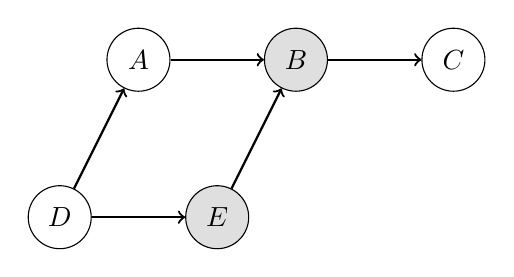
\begin{tikzpicture}[
        observed/.style={circle, draw=black!100, fill=gray!25, minimum size=8mm},
        hidden/.style={circle, draw=black!100, fill=white, minimum size=8mm}]

        \node[hidden] (A) at (0, 0) {$A$};
        \node[observed] (B) at (2, 0) {$B$};
        \node[hidden] (C) at (4, 0) {$C$};
        \node[hidden] (D) at (-1, -2) {$D$};
        \node[observed] (E) at (1, -2) {$E$};

        \draw[->, thick] (A) -- (B);
        \draw[->, thick] (B) -- (C);
        \draw[->, thick] (D) -- (A);
        \draw[->, thick] (D) -- (E);
        \draw[->, thick] (E) -- (B);
    \end{tikzpicture}
\end{center}
\begin{itemize}
    \item ${\bf P}(A | b, e) \propto \sum_c \sum_d P(c|b) {\bf P}(b | A) P(b|e) {\bf P}(A | d) P(e|d) P(d)$
    \item ${\bf P}(A | b, e) \propto \sum_c \sum_d P(c|b) {\bf P}(b | A, e) {\bf P}(A|d) P(e|d)$
    \solitem ${\bf P}(A | b, e) \propto \sum_c \sum_d P(c|b) {\bf P}(b | A, e) {\bf P}(A | d) P(e|d) P(d)$ %%%
    \item ${\bf P}(A | b, e) \propto \sum_b \sum_e P(c | b) {\bf P}(A | b,e) {\bf P}(A | d) P(e|d) P(d)$
\end{itemize}

In a Bayesian network
\begin{itemize}
    \solitem Independence between two variables is guaranteed if all path connecting them are inactive.
    \item We can guarantee dependence between two variables using d-separation.
    \item A path between two nodes is active if it contains at least one active triplet.
    \item A cascade triplet is active if the center node is observed.
\end{itemize}

In a one node Bayesian network with a binary variable following a Bernoulli distribution. If we observe $T$ positive realizations and $F$ negative ones,
\begin{itemize}
    \item the maximum likelihood estimate of the positive probability is $\dfrac{T}{F}$.
    \item the maximum likelihood estimate of the positive probability is $\dfrac{T + F}{T}$.
    \solitem the maximum likelihood estimate of the positive probability is $\dfrac{T}{T + F}$.
    \item None of the above.
\end{itemize}

\end{document}